\chapter{Motion Planning}
\label{chap:Motion_planning}

"Motion planning (also known as the navigation problem or the piano mover's problem) is a term used in robotics for the process of breaking down a desired movement task into discrete motions that satisfy movement constraints and possibly optimize some aspect of the movement.
A basic motion planning problem is to produce a continuous motion that connects a start configuration \texttt{S} and a goal configuration \texttt{G}, while avoiding collision with known obstacles. The robot and obstacle geometry is described in a 2D or 3D workspace, while the motion is represented as a path in (possibly higher-dimensional) configuration space"\cite{wiki_motion_planning}.

\texttt{Configuration space}\\
Although the motion planning problem is applied in the real world, in computer science we need to convert the real space into another space: \texttt{configuration space}.

"A configuration describes the pose of the robot, and the configuration space \texttt{C} is the set of all possible configurations"\cite{wiki_motion_planning}.

According to the definition of configuration space we know that a robot configuration is a specification of the positions of all robot points relative to a fixed coordinate system. And in our case the robot only moves on the ground which means the workspace is a 2-dimensional plane and currently we do not consider translation and rotation of the robot, we can treat the robot as a singe point(zero-sized) translating in this 2-dimensional workspace \texttt{C}, and the configuration can be represented with two parameters (x, y).  

\begin{figure}[h]
\centering
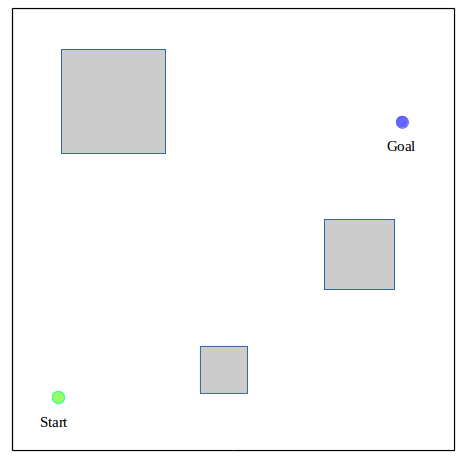
\includegraphics[scale=0.5]{./fig/confi_space.png}
\caption{Configuration space of a point-sized robot. White = $C_{free}$, gray = $C_{obs}$, green point = Start, blue point = Goal\cite{wiki_motion_planning}.}
\label{fig:confi_space}
\end{figure}

\texttt{Grid-based search}\\
For path planning the continuous terrain needs to be discretized, so we need to use some methods to discretize the configuration space. Because of low-dimensional of our workplace and the grid-based algorithm is known as one of common approaches in robotics, the configuration space can be planed on a 2D occupancy grid map, which means we can overlay a grid on top of configuration space.

"Grid-based approaches overlay a grid on configuration space, and assume each configuration is identified with a grid point. At each grid point, the robot is allowed to move to adjacent grid points as long as the line between them is completely contained within $C_{free}$ (this is tested with collision detection)"\cite{wiki_motion_planning}.

If we use grid-based approaches, a grid resolution is required to set. In addition to this, we also need to consider the width and height of the grid, e.g. if we assume that the camera's detection region is a half circle with radius 3 meters, we can set the grid as a $3m \times 6m$ square. This gird is shown in figure \ref{fig:grid_world_marker}. 

\begin{figure}[h]
\centering
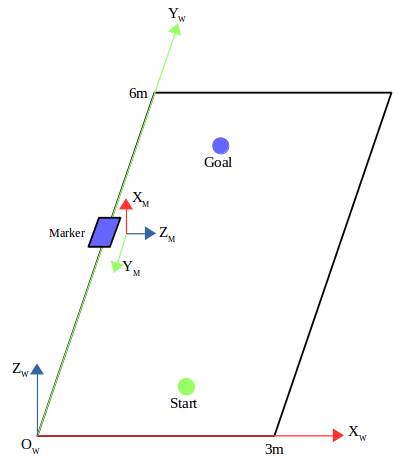
\includegraphics[scale=0.6]{./fig/grid_world_marker.png}
\caption{Convert configuration space into a $3m \times m$ grid. The center of the marker is at $(0,3m)$ in world coordinates}
\label{fig:grid_world_marker}
\end{figure}

There are so many known search algorithms which can be applied in different cases, in our simulation we applied \texttt{A*} and \texttt{Artificial potential fields} as our search algorithm and we compared the accuracy of the paths which are computed with these two algorithm. In following sections I will describe the details how to apply the regular \texttt{A*} search algorithm and \texttt{Artificial potential fields} related to our condition number distribution in our situation.

\section{The selected pose estimation algorithm}
In our simulations in order to compute the measured path four different pose estimation algorithms were performs. And we compared the rotational error and translational error of each algorithm for our camera distribution on YZ-plane of marker coordinates. The error results are shown in figure \ref{fig:r_error_and_t_error_ippe}, figure \ref{fig:r_error_and_t_error_lm} and figure \ref{fig:r_error_and_t_error_dls}. Therefrom we found that the iterative method based on the Levenberg-Marquardt optimization denoted as \texttt{LM} has the relative smaller R-error and t-error than others. Therefore we applied \texttt{LM} as our pose estimation algorithm for \texttt{A*} and artificial potential fields method.
\begin{figure}[H]
\centering
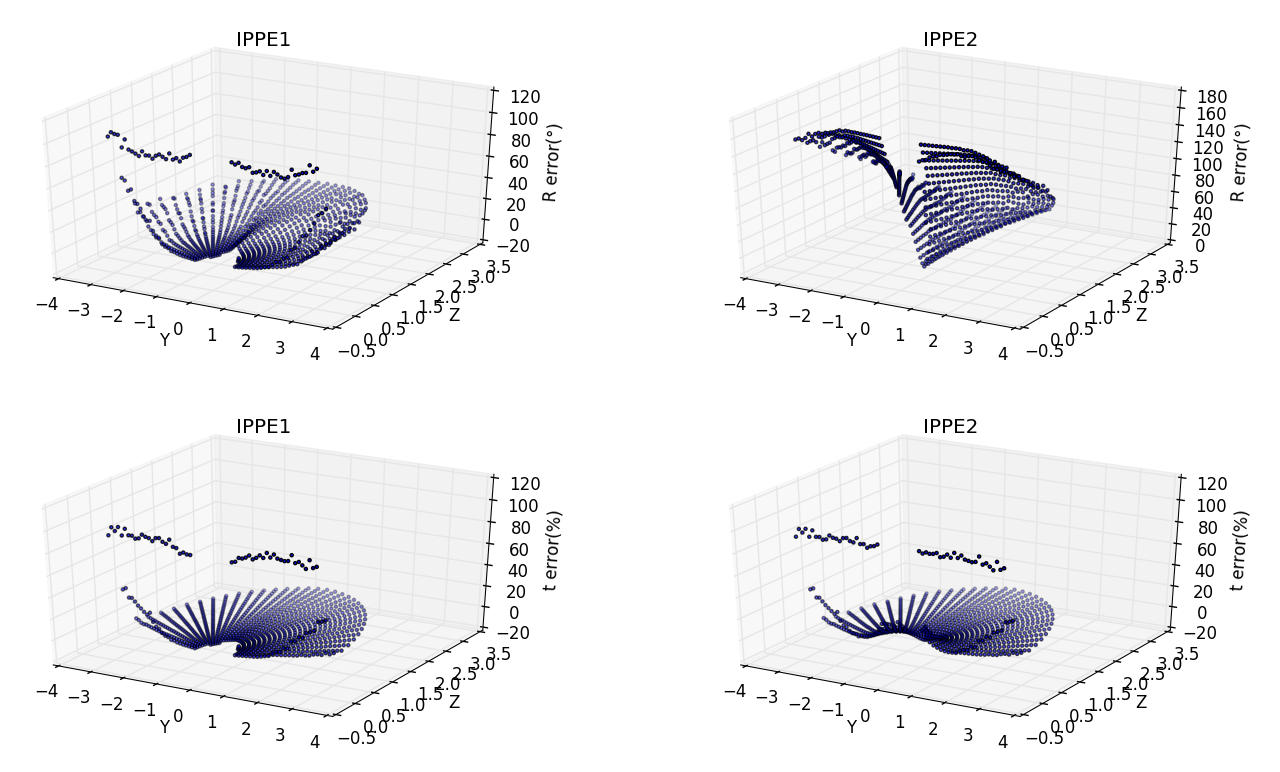
\includegraphics[scale=0.5]{./fig/r_error_and_t_error_ippe.png}
\caption{Rotational error and translational error for the selected \texttt{IPPE} method\cite{collins2014infinitesimal}}
\label{fig:r_error_and_t_error_ippe}
\end{figure}

\begin{figure}[H]
\hspace*{1.5cm}
\centering
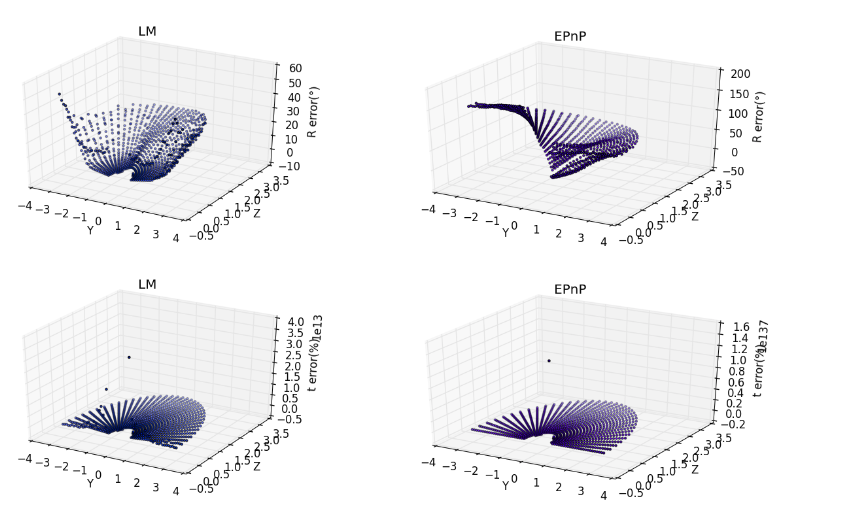
\includegraphics[scale=0.8]{./fig/r_error_and_t_error_ippe_lm.png}
\caption{Rotational error and translational error for the selected \texttt{LM} and \texttt{EPnP} methods\cite{lepetit2009epnp}}
\label{fig:r_error_and_t_error_lm}
\end{figure}

\begin{figure}[H]
\centering
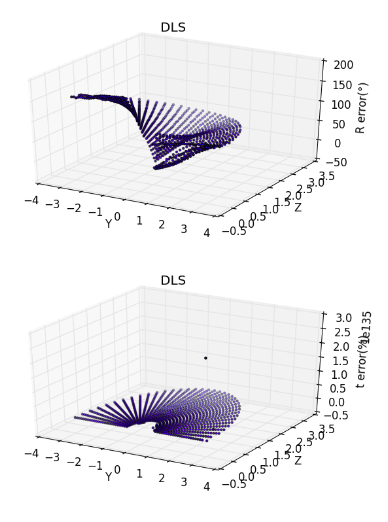
\includegraphics[scale=0.8]{./fig/r_error_and_t_error_ippe_dls.png}
\caption{Rotational error and translational error for the selected \texttt{DLS} method}
\label{fig:r_error_and_t_error_dls}
\end{figure}


\section{A* search algorithm}
\texttt{A*} is a widely used informed search algorithm in pathfinding. In our situation we applied the regular \texttt{A*} algorithm without considering the condition number distribution and collision avoidance problem in workspace to compute the least cost path, which means the actual shortest path from start node to goal node.

We know that \texttt{A*} is based on an estimate of the cost(total weight) from start node to goal node. Specifically, \texttt{A*} selects the path that minimizes:
\begin{align*}
\Aboxed{f(n) = g(n) + h(n)}
\end{align*}
where n is the current node, g(n) is the cost of the path from the start node to n, and h(n) is a heuristic that estimates the cost of the cheapest path from n to the goal, f(n) is the total cost of the current node. \texttt{A*} computes $f(n) = g(n) + h(n)$. To add two values, those two values need to be at the same scale.

Because the heuristic is problem-specific\cite{wiki_A} and on a grid, there are some well-known heuristic functions to use e.g. \texttt{manhattan distance}, \texttt{diagonal distance}, \texttt{euclidean distance} and so on. And considering that in our situation the robot can move in 8 directions on the given square grid, therefore \texttt{diagonal distance} is suitable for our situation. The following shows how to compute the \texttt{diagonal distance}:
\begin{align*}
dx &= abs(node.x - goal.x)\\
dy &= abs(node.y - goal.y) \\
h &= D * (dx + dy) + (D2 - 2 * D) * min(dx, dy)
\end{align*}
where \texttt{D} is the minimum cost of moving from one space to an adjacent space horizontally or vertically and \texttt{D2} is the cost of moving diagonally. And we set $D = 10$ and $D2 = 14$ in our simulation, we take these values because the distance along the diagonal line is $\sqrt{2}$ or about 1.414 times that it takes to move horizontally or vertically. For simplicity, we use 10 and 14 approximations avoiding to calculate the root and decimals. Using such integers is also faster for calculation of computers.

\begin{figure}[h]
\centering
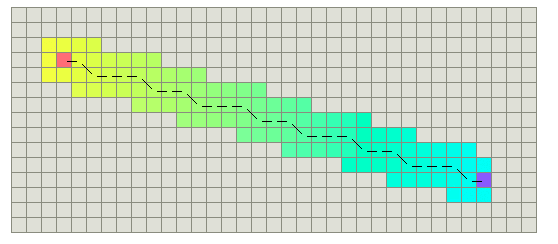
\includegraphics[scale=1]{./fig/Astar.png}
\caption{Calculated path with \texttt{A*} search algorithm on grid. The robot can move in 8 directions(\texttt{Diagonal distance} as heuristic function)\cite{AHeuristic}.}
\label{fig:Astar}
\end{figure}

The following pseudocode describes the \texttt{A*} algorithm\cite{wiki_A}:
\begin{algorithmHu}[caption={A* pseudocode}, label={alg1}]
 input: start node, goal node
 output: least cost path from start to goal
 
 Initial:
        openList = {start}
        closedList := {}
        cameFrom := {}
        g(start) := 0
        h(start) := heuristic_function(start, goal)
        f(start) := g(start) + h(start)
        
 while openList is not empty:
        current := the node in openList with the lowest f value  
        if current = goal
           return
        remove current from openList
        add current to closedList
        
        for each neighbor of current
             if neighbor in closedList
                continue
             
             if neighbor not in openList
                add neighbor to openList
                
             tentative_g := g(current) + dist_between(current, neighbor)    
             if tentative_g >= g(neighbor)
                continue   
                    
             cameFrom(neighbor) := current
             g(neighbor) := tentative_g 
             f(neighbor) := g(neighbor) + heuristic_function(neighbor, goal)
 return failure  
        
\end{algorithmHu}

The key to find the shortest path(optimal solution) is how to select the heuristic function $h(n)$\cite{AHeuristic}: 
\begin{itemize}
\item If h(n) is 0, \texttt{A*} turns into Dijkstra's Algorithm.
\item If h(n) is always lower than(or equal to) the cost of moving from n to the goal, in this case the lower $h(n)$ is, the more nodes \texttt{A*} expands, low efficiency(slower). However \texttt{A*} is guaranteed to find a shortest path.
\item If h(n) is exactly equal to the cost of moving from n to the goal, \texttt{A*} will find the shortest path and the search will be strictly along the shortest path. The search efficiency at this time is the highest.
\item If h(n) is greater than the cost of moving from n to the goal, the number of search points is few, the search range is small, and the efficiency is high, but the optimal solution cannot be guaranteed.
\item If h(n) is very high compared to g(n), \texttt{A*} turns into Greedy Best-First-Search.
\end{itemize}

In future work, we will modify the \texttt{A*} search algorithm adding condition number to heuristic function and adding obstacles in grid(considering the problem of collision avoidance). Subsequently, comparing the accuracy of paths with modified \texttt{A*} and artificial potential fields method.

\section{Artificial potential fields}

"One approach is to treat the robot's configuration as a point (usually electron) in a potential field that combines attraction to the goal, and repulsion from obstacles. The resulting trajectory is output as the path.The Artificial potential fields can be achieved by direct equation similar to electrostatic potential fields or can be drive by set of linguistic rules"\cite{wiki_motion_planning}.

The artificial potential fields include the attractive fields and repulsive fields. The target point(goal) generates attractive force on the object and guides the object moving toward it. The obstacles generate repulsive force on the object and prevent the object from colliding with them. The total force of an object at each point in the path is equal to the sum of all attractive forces and repulsive forces at that point.
\begin{align*}
\Aboxed{ 
U(q) = U_{att}(q) + U_{rep}(q)
}
\end{align*}

\begin{figure}[H]
\centering
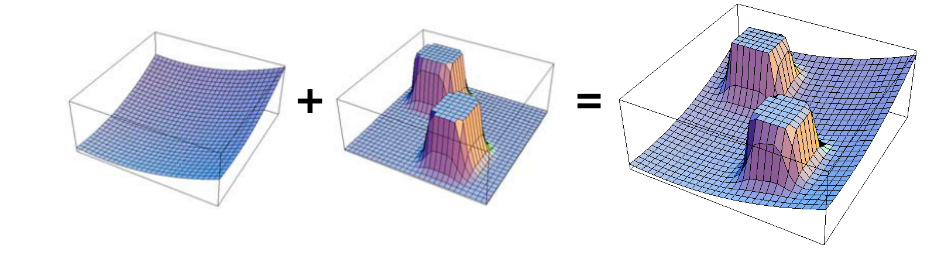
\includegraphics[scale=0.6]{./fig/apf.png}
\caption{Attractive potential fields + repulsive potential fields = Total potential fields\cite{choset2010robotic}}
\label{fig:apf}
\end{figure}

The key of artificial potential fields method is how to construct the attractive fields and the repulsive fields. In our situation we did not consider the obstacles on the gird temporarily, but we treated the condition number distribution on the grid as repulsive fields. 
In our case the order of condition number is 1 to 10, therefore the order of the attractive potential should be less than $10^2$. This is because if the values of the attractive potential are much larger than the condition numbers, only the attractive potential plays the role and the robot would not be affected by the repulsive potential fields(condition number distribution). The following shows our used attractive potential function and repulsive potential function:
\begin{align*}
U_{att}(q) &= \frac{1}{2} \zeta d(q,q_{goal}) \\
U_{rep}(q) &= \text{condition number distribution on grid}
\end{align*}
where, $\zeta$ is a positive scaling factor, $d(q, q_{goal})$ is the distance between the robot q and the goal $q_{goal}$. We set $\zeta = 5$ in our simulation in order to get similar orders of attractive potential and condition number.


\begin{figure}[H]
\centering
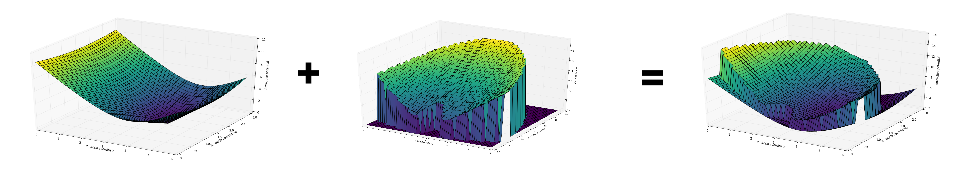
\includegraphics[scale=0.6]{./fig/combine.png}
\caption{Artificial potential fields method in our situation, in this figure the start is $(1.55m,2.05m)$ and the goal is $(1.55m,4.05m)$.}
\label{fig:combine}
\end{figure}

\begin{figure}[h]
  \centering
  \begin{subfigure}[b]{0.75\textwidth}
    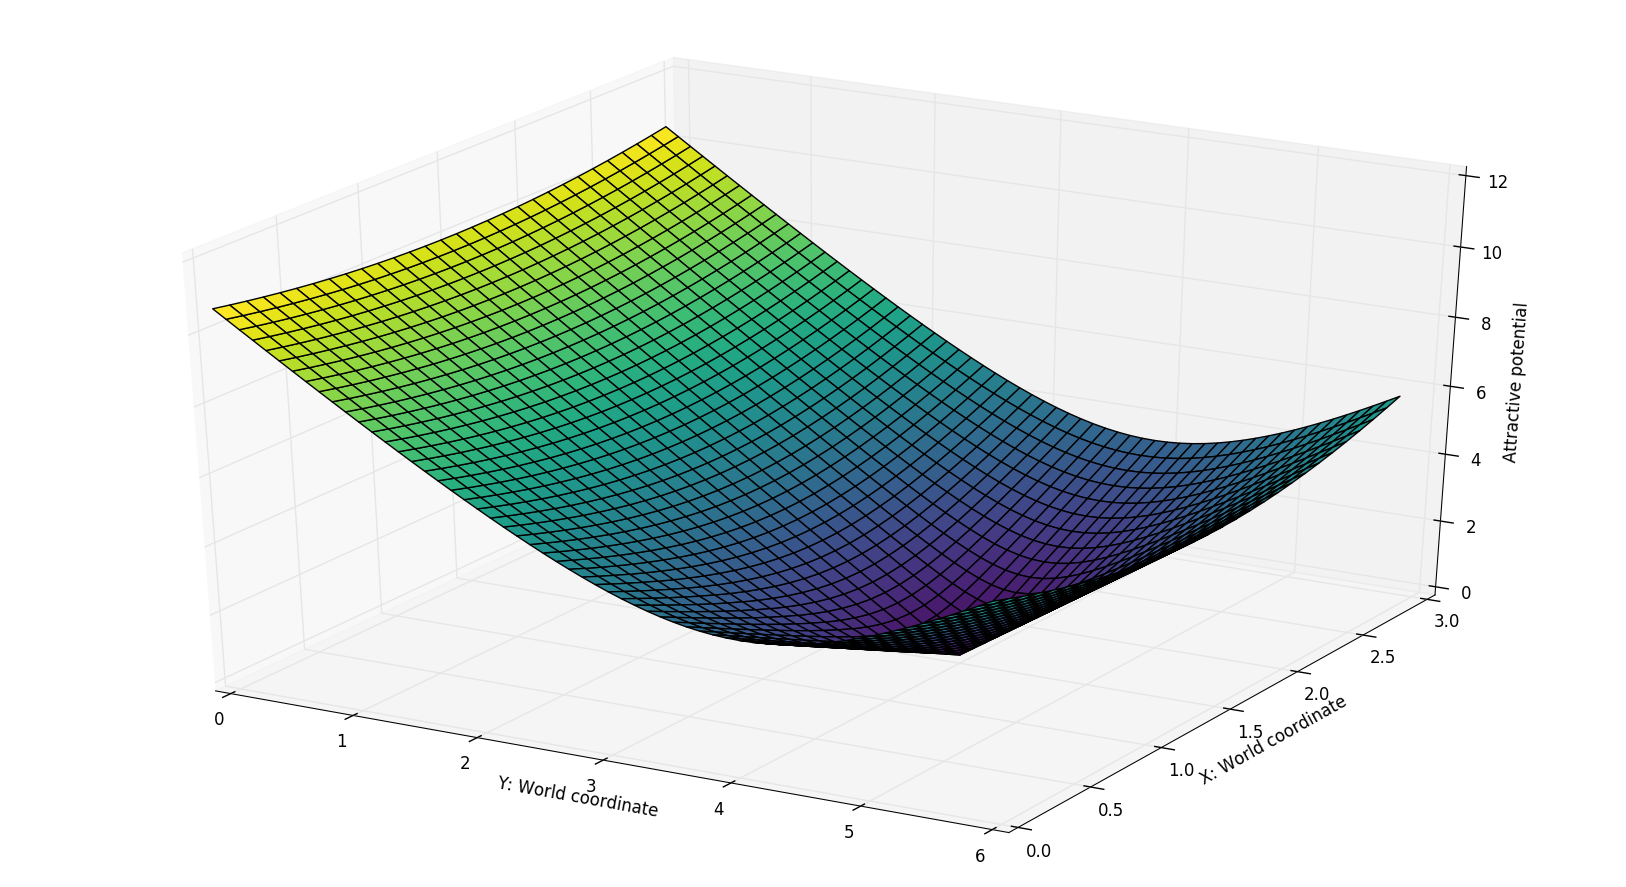
\includegraphics[width=\textwidth]{./fig/Attractive_potential.png}
    \caption{Attractive potential fields}
  \end{subfigure}
  \begin{subfigure}[b]{0.75\textwidth}
    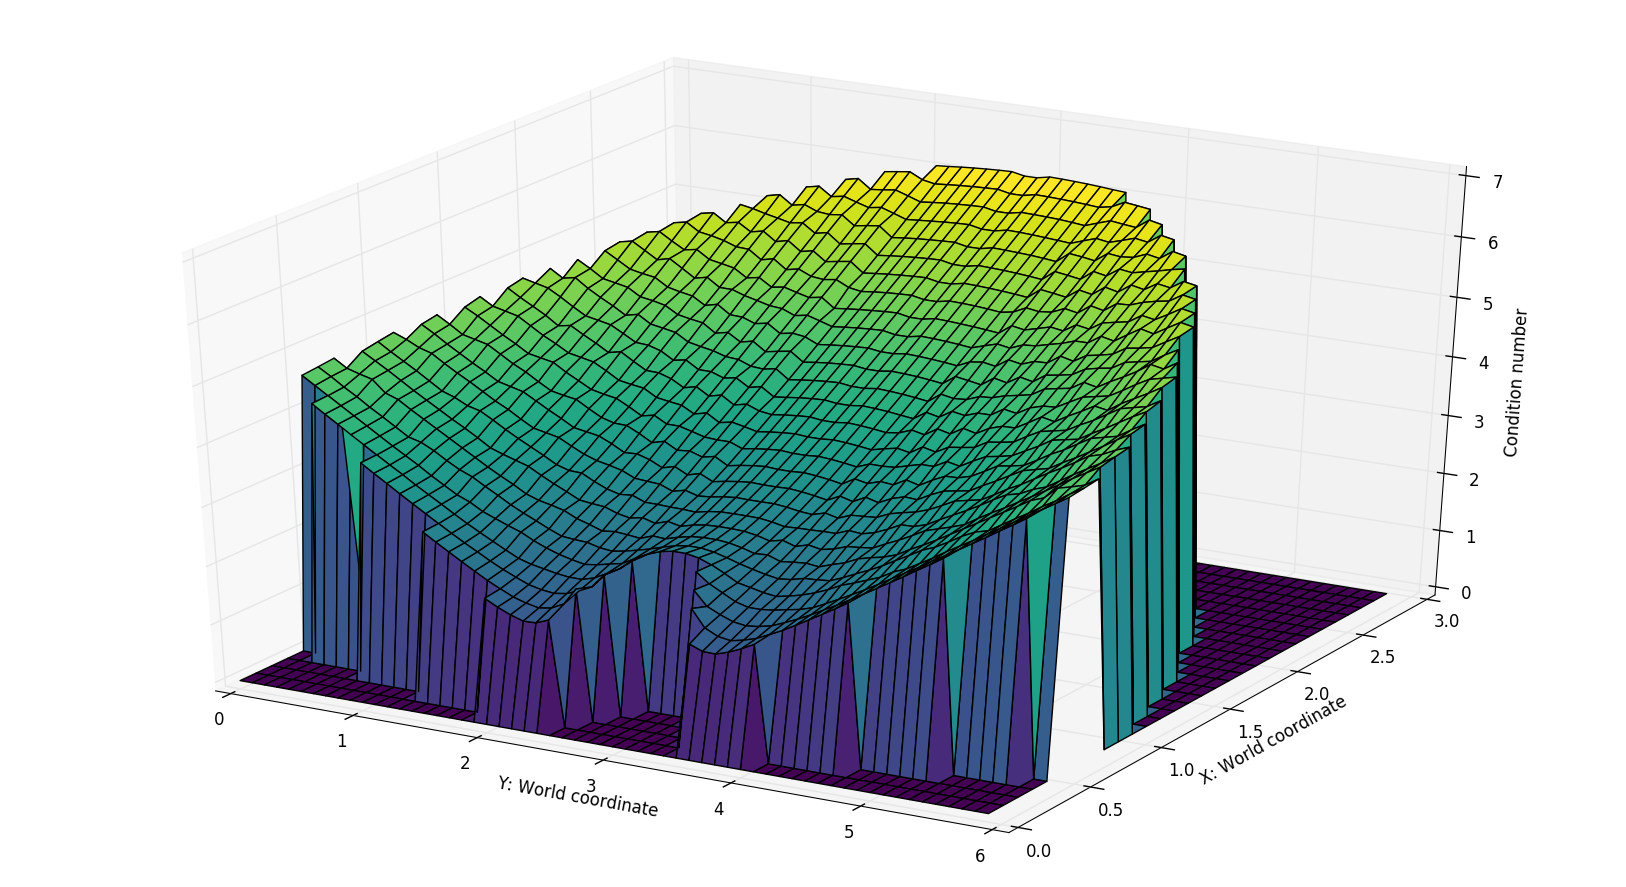
\includegraphics[width=\textwidth]{./fig/condNum3Dbig.png}
    \caption{Condition number distribution as repulsive potential fields}
  \end{subfigure}
  \begin{subfigure}[b]{0.75\textwidth}
    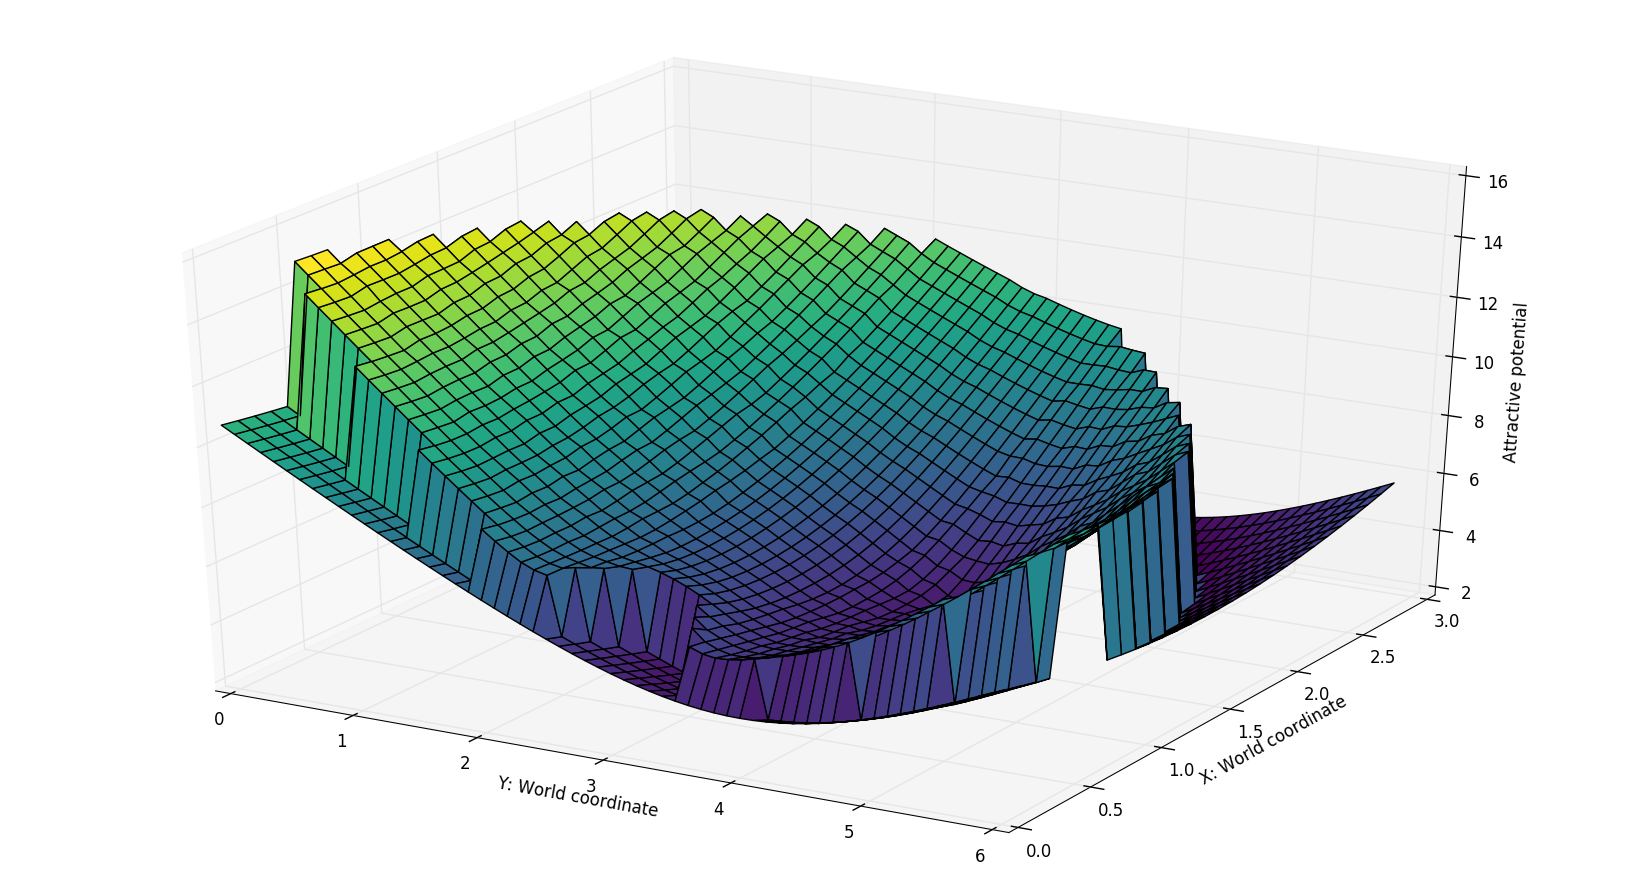
\includegraphics[width=\textwidth]{./fig/total_potential.png}
    \caption{Total potential fields}
  \end{subfigure}
  \caption{Artificial potential fields method in our situation}
  \label{fig:total_potential}
\end{figure}

The artificial potential fields method has advantages in that it's has simple structure, easy to implement the underlying real-time control and the path is produced with little computation. However, when the attractive force and repulsive force has similar value but on the opposite direction, the total potential force of the robot would be zero, then it will cause robot to be trapped in local minima or oscillations and fail to find a path\cite{RoboTemad2}\cite{wiki_motion_planning}.


\section{Compare accuracy of paths calculated with A* and artificial potential fields method}

In our simulations we set the grid as a $3m \times 6m$ square and the resolution of the grid as 0.1m. The Iterative method based on Levenberg-Marquardt optimization as the pose estimation algorithm was run at each iteration\cite{SOLVEPNP_ITERATIVE}.
Two desired paths, one was computed with \texttt{A*}, another was computed with artificial potential fields method are shown in figure \ref{fig:comparePaths}.
\begin{figure}[H]
\centering
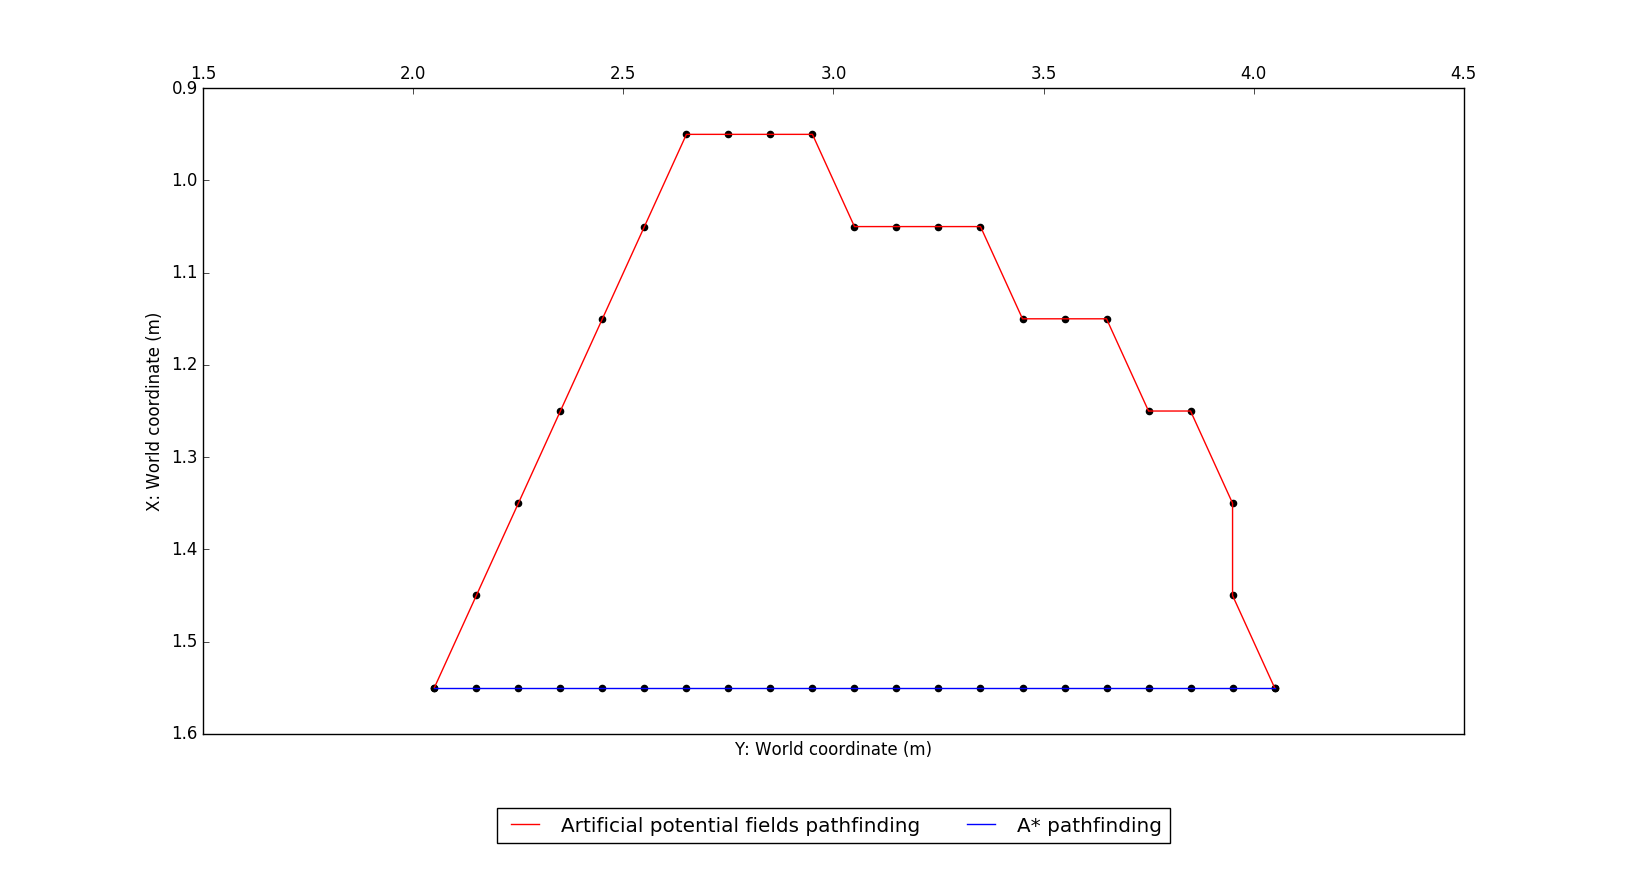
\includegraphics[scale=0.3]{./fig/comparePaths.png}
\caption{Start point: (1.55m,2.05m), goal point: (1.55m,4.05m). The center of the planar marker is at (0,3m). Blue line: path computed with \texttt{A*}, red line: path computed with artificial potential fields method. Each point means each step on the path.}
\label{fig:comparePaths}
\end{figure}

For each desired path, 100 times simulation of the measured paths were performs. For each iteration, 1000 runs of the pose estimation of each step on the desired path were performed. We calculated the mean and standard derivation of errors(euclidean distance) of these 100 times iterations. 
In figure \ref{fig:comparePathsError} the intervals are built from the mean error of each step, we can find that the errors of the path computed with \texttt{A*} are obviously larger than the path computed with artificial potential fields method. Figure \ref{fig:distanceErrorMayavi} represents the comparison of two paths with another form, we can still notice that the errors of these two paths have huge differences, the path computed with artificial potential fields method is more accurate then the path computed with \texttt{A*}.

\begin{figure}[H]
\centering
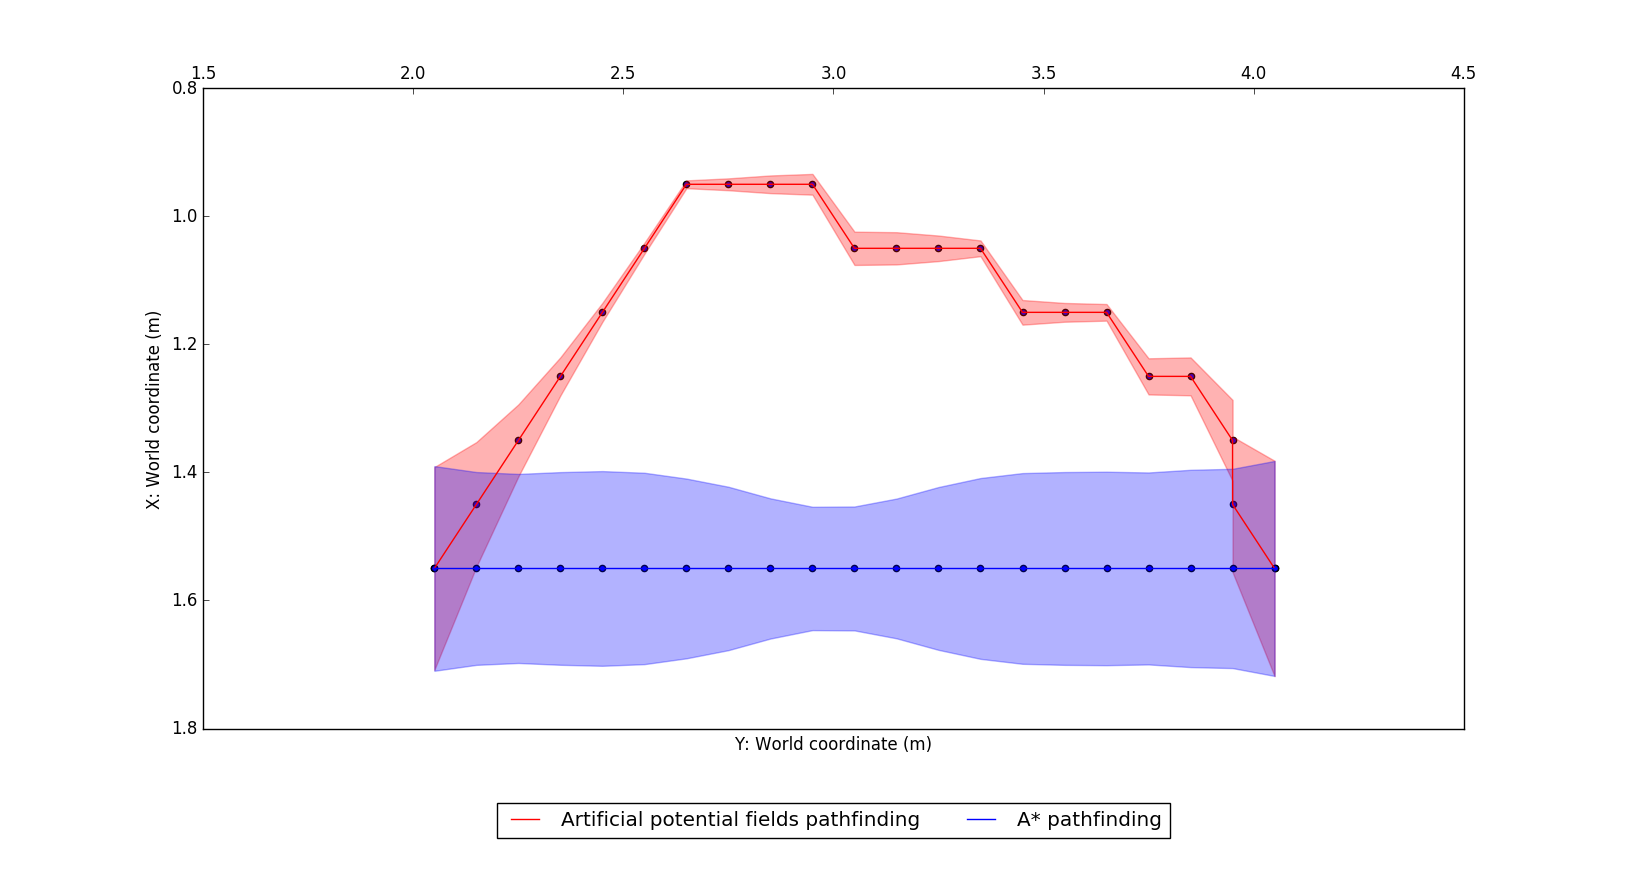
\includegraphics[scale=0.3]{./fig/comparePathsError.png}
\caption{The blue intervals and red intervals represent the mean error(euclidean distance) between desired paths and measured paths}
\label{fig:comparePathsError}
\end{figure}


\begin{figure}[H]
\centering
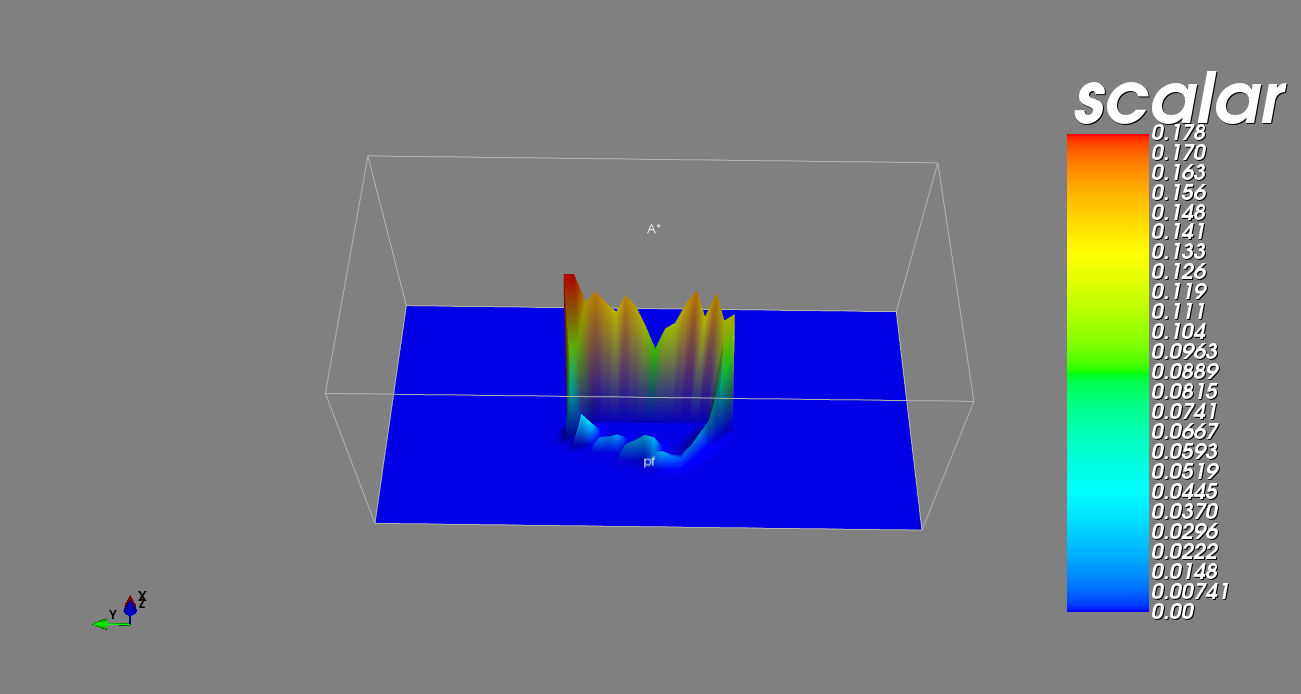
\includegraphics[scale=0.3]{./fig/distanceErrorMayavi.png}
\caption{Compare the errors of paths computed with \texttt{A*} and artificial potential fields method}
\label{fig:distanceErrorMayavi}
\end{figure}

We also compared the errors of both paths with it's mean and it's standard deviation in figure \ref{fig:distanceError}. It is obviously to notice that the mean error value and standard deviation on path computed with artificial potential fields method are smaller than that on path computed with \texttt{A*} almost at each step. 

%------------------------R T error-----------------------------
Sequentially the rotational error and translational error of both paths were compared which are shown in figure \ref{fig:compareRErrortError}. We can find that the path computed with artificial potential fields method has a smaller rotational error and translational error than the path computed with \texttt{A*} almost at each step. Another form to represent the comparisons of rotational error and translational error are shown in figure \ref{fig:RErrorMayavi} and \ref{fig:tErrorMayavi}.

\begin{figure}[H]
\centering
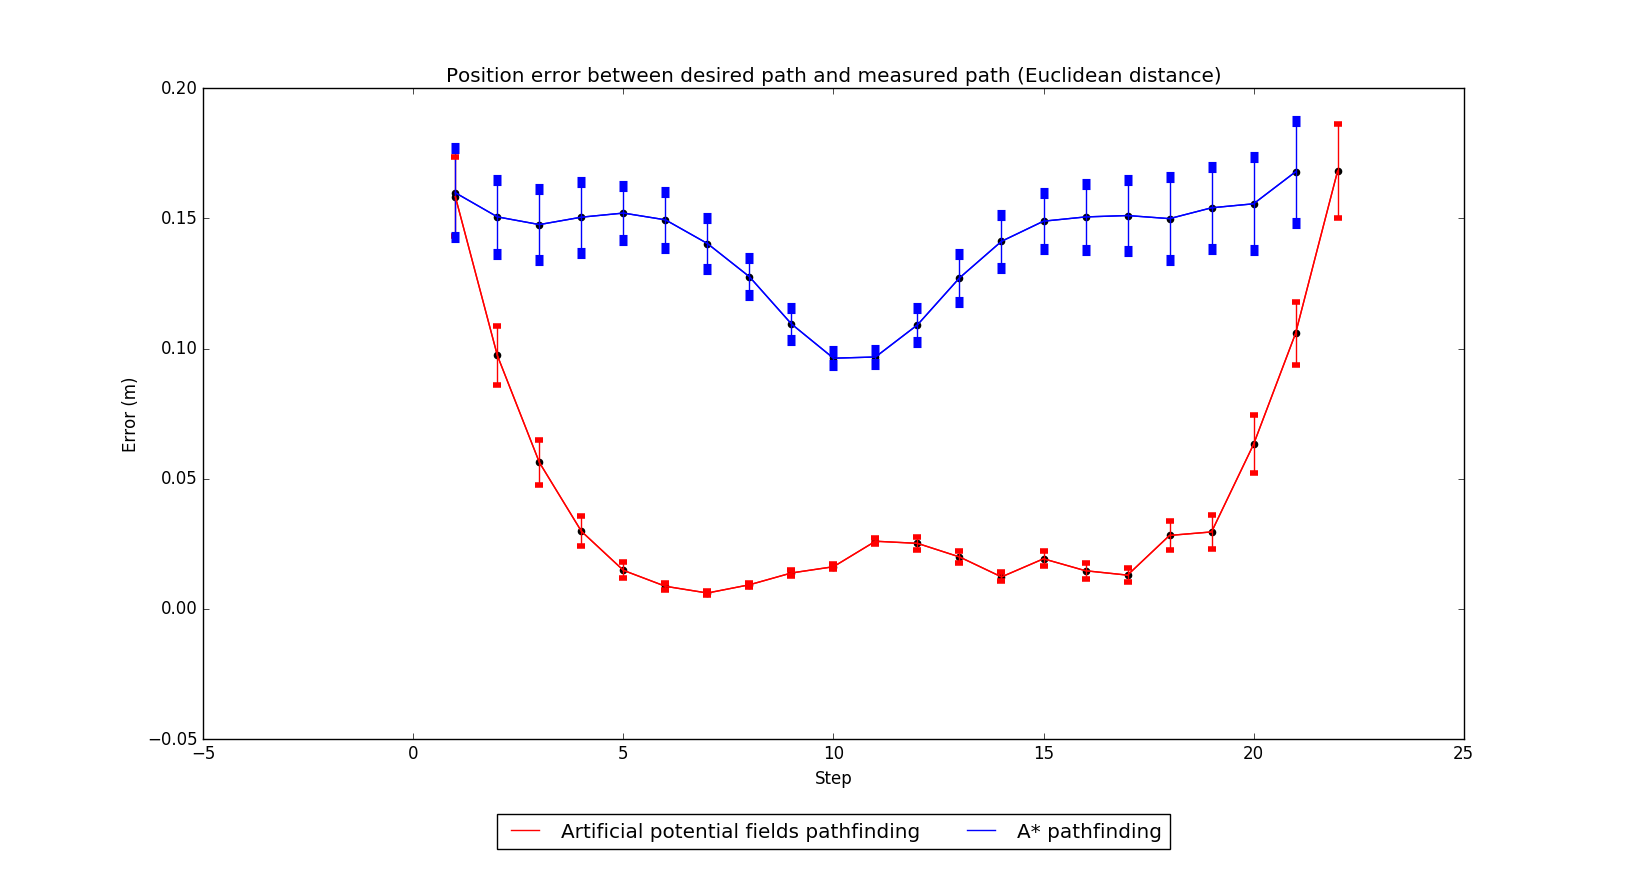
\includegraphics[scale=0.3]{./fig/distanceError.png}
\caption{Blue line: Mean error of \texttt{A*} computed path, red line: mean error of artificial potential fields computed path. At each point represents the standard deviation of the error.}
\label{fig:distanceError}
\end{figure}

\begin{figure}[H]
\centering
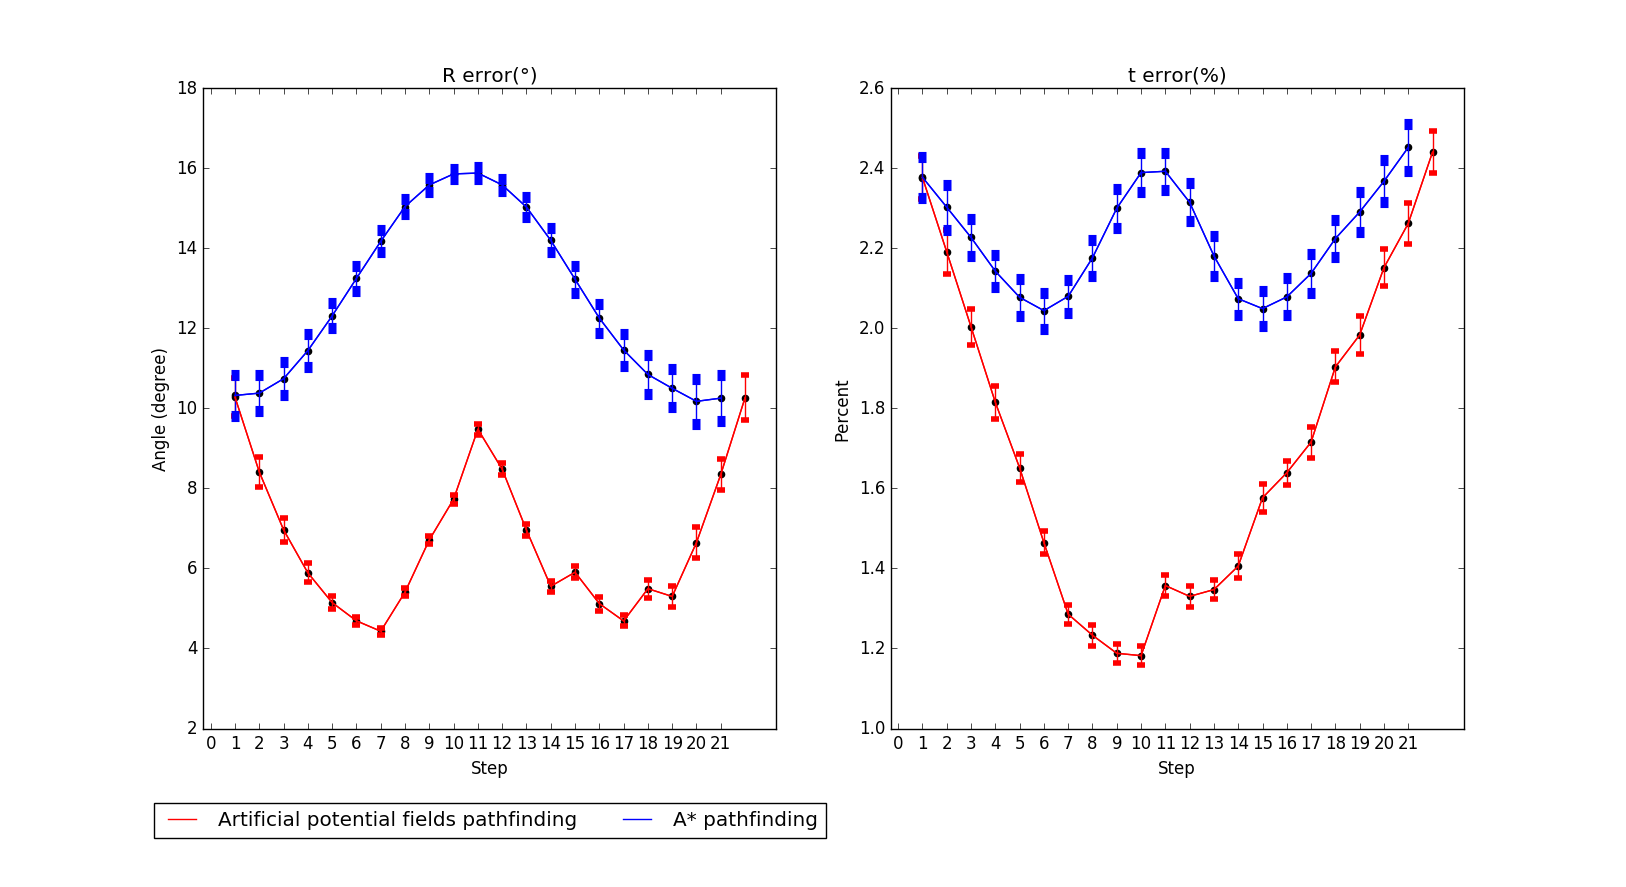
\includegraphics[scale=0.3]{./fig/compareRErrortError.png}
\caption{Blue line: Rotational error and translational error of path computed with \texttt{A*}, red line: Rotational error and translational error of path computed with artificial potential fields method. At each point represents the error standard deviation.}
\label{fig:compareRErrortError}
\end{figure}

\begin{figure}[H]
\centering
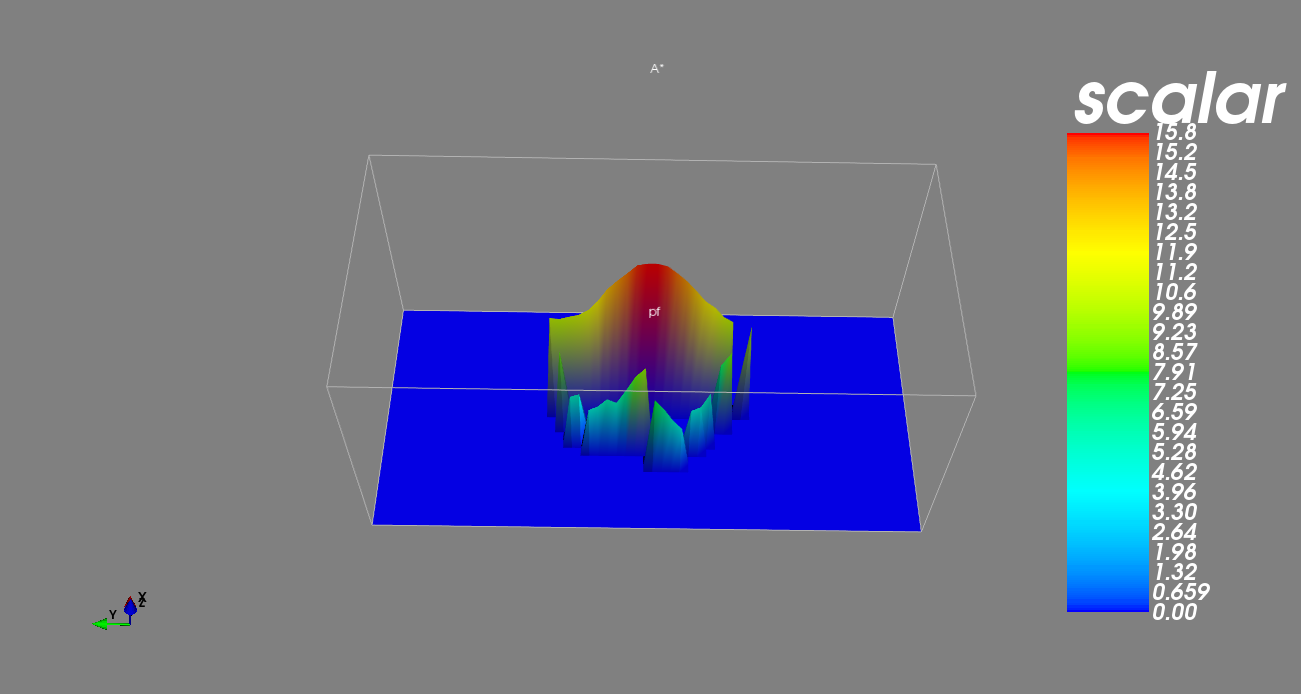
\includegraphics[scale=0.3]{./fig/RErrorMayavi.png}
\caption{Compare the rotational errors of paths computed with \texttt{A*} and artificial potential fields method}
\label{fig:RErrorMayavi}
\end{figure}

\begin{figure}[H]
\centering
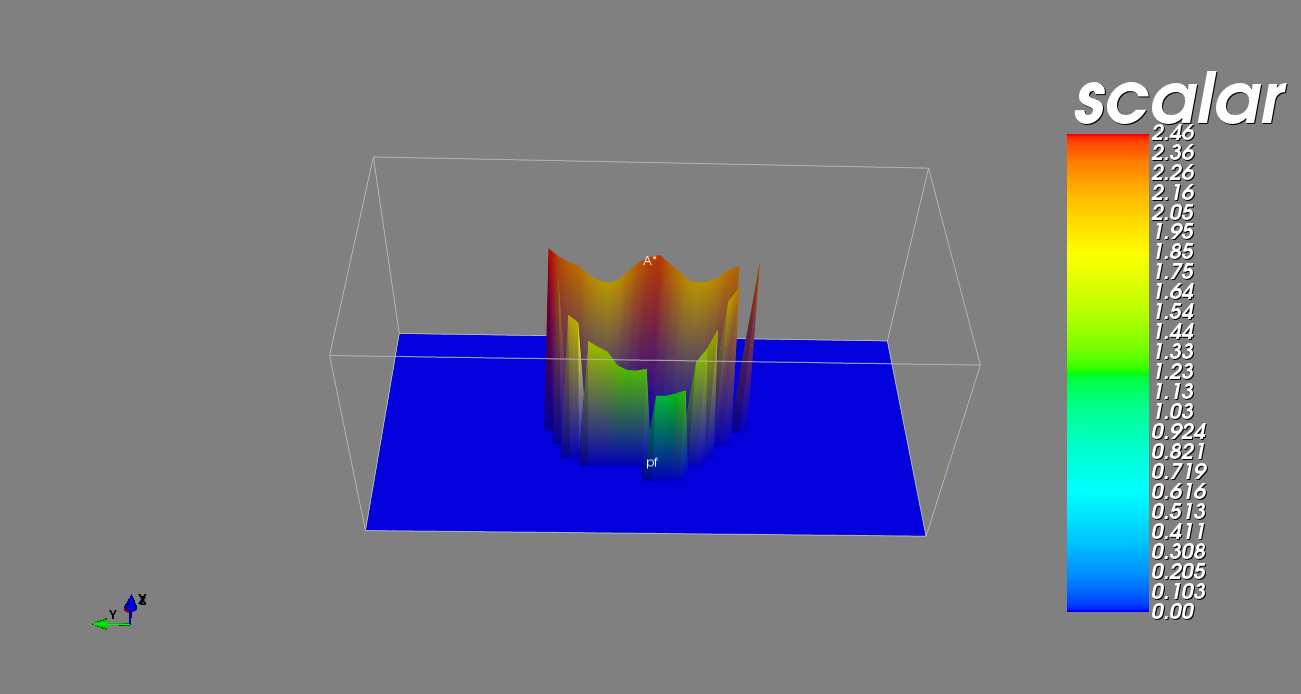
\includegraphics[scale=0.3]{./fig/tErrorMayavi.png}
\caption{Compare the translational errors of paths computed with \texttt{A*} and artificial potential fields method}
\label{fig:tErrorMayavi}
\end{figure}



